\documentclass[superscriptaddress,onecolumn,floatfix]{revtex4-2}

\usepackage{graphicx}
\usepackage{epsfig}
\usepackage{color}
\usepackage{amssymb}
\usepackage{amsmath}
\usepackage{array}
\usepackage[loose]{units}
\usepackage[english]{babel}
\usepackage[unicode]{hyperref}
\usepackage{cleveref}
\usepackage{braket}
\usepackage[caption=false]{subfig}
\usepackage{letltxmacro}

\pdfcompresslevel=9

\LetLtxMacro{\ORIGselectlanguage}{\selectlanguage}
\makeatletter
\DeclareRobustCommand{\selectlanguage}[1]{%
    \@ifundefined{alias@\string#1}
      {\ORIGselectlanguage{#1}}
      {\begingroup\edef\x{\endgroup
         \noexpand\ORIGselectlanguage{\@nameuse{alias@#1}}}\x}%
}
\newcommand{\definelanguagealias}[2]{%
  \@namedef{alias@#1}{#2}%
}
\makeatother

\definelanguagealias{en}{english}


\begin{document}
                            
\begin{abstract}
  This guide walks you through the steps needed to install the Selectable CAN harness in your 2021-2024 Ioniq 5. See also the \href{https://youtube.com/playlist?list=PLYCTmVJH4UYqnw87UZAaqMo1GrOv0cJaL}{video guides}:
  \begin{description}
    \item[Step 1: Disconnect 12V] \href{https://youtu.be/ePBdyeBYKk4}{video guide}
    \item[Step 2: Install Harness] \href{https://youtu.be/kVvkR4ZLFMI}{harness intall guide}
  \end{description}
\end{abstract}
\title{Selectable CAN install guide}
\author{Electroniq Buttons Boutique}
\email{support@electroniqbuttons.com}
% \affiliation{\GOE}
% \author{Benjamin J. McMorran}
% \email{mcmorran@uoregon.edu}
% \affiliation{\UO}
\date{\today}

\maketitle

% \begin{figure}[h]
%   \subfloat[]{\label{subfig:overview:harness}
%   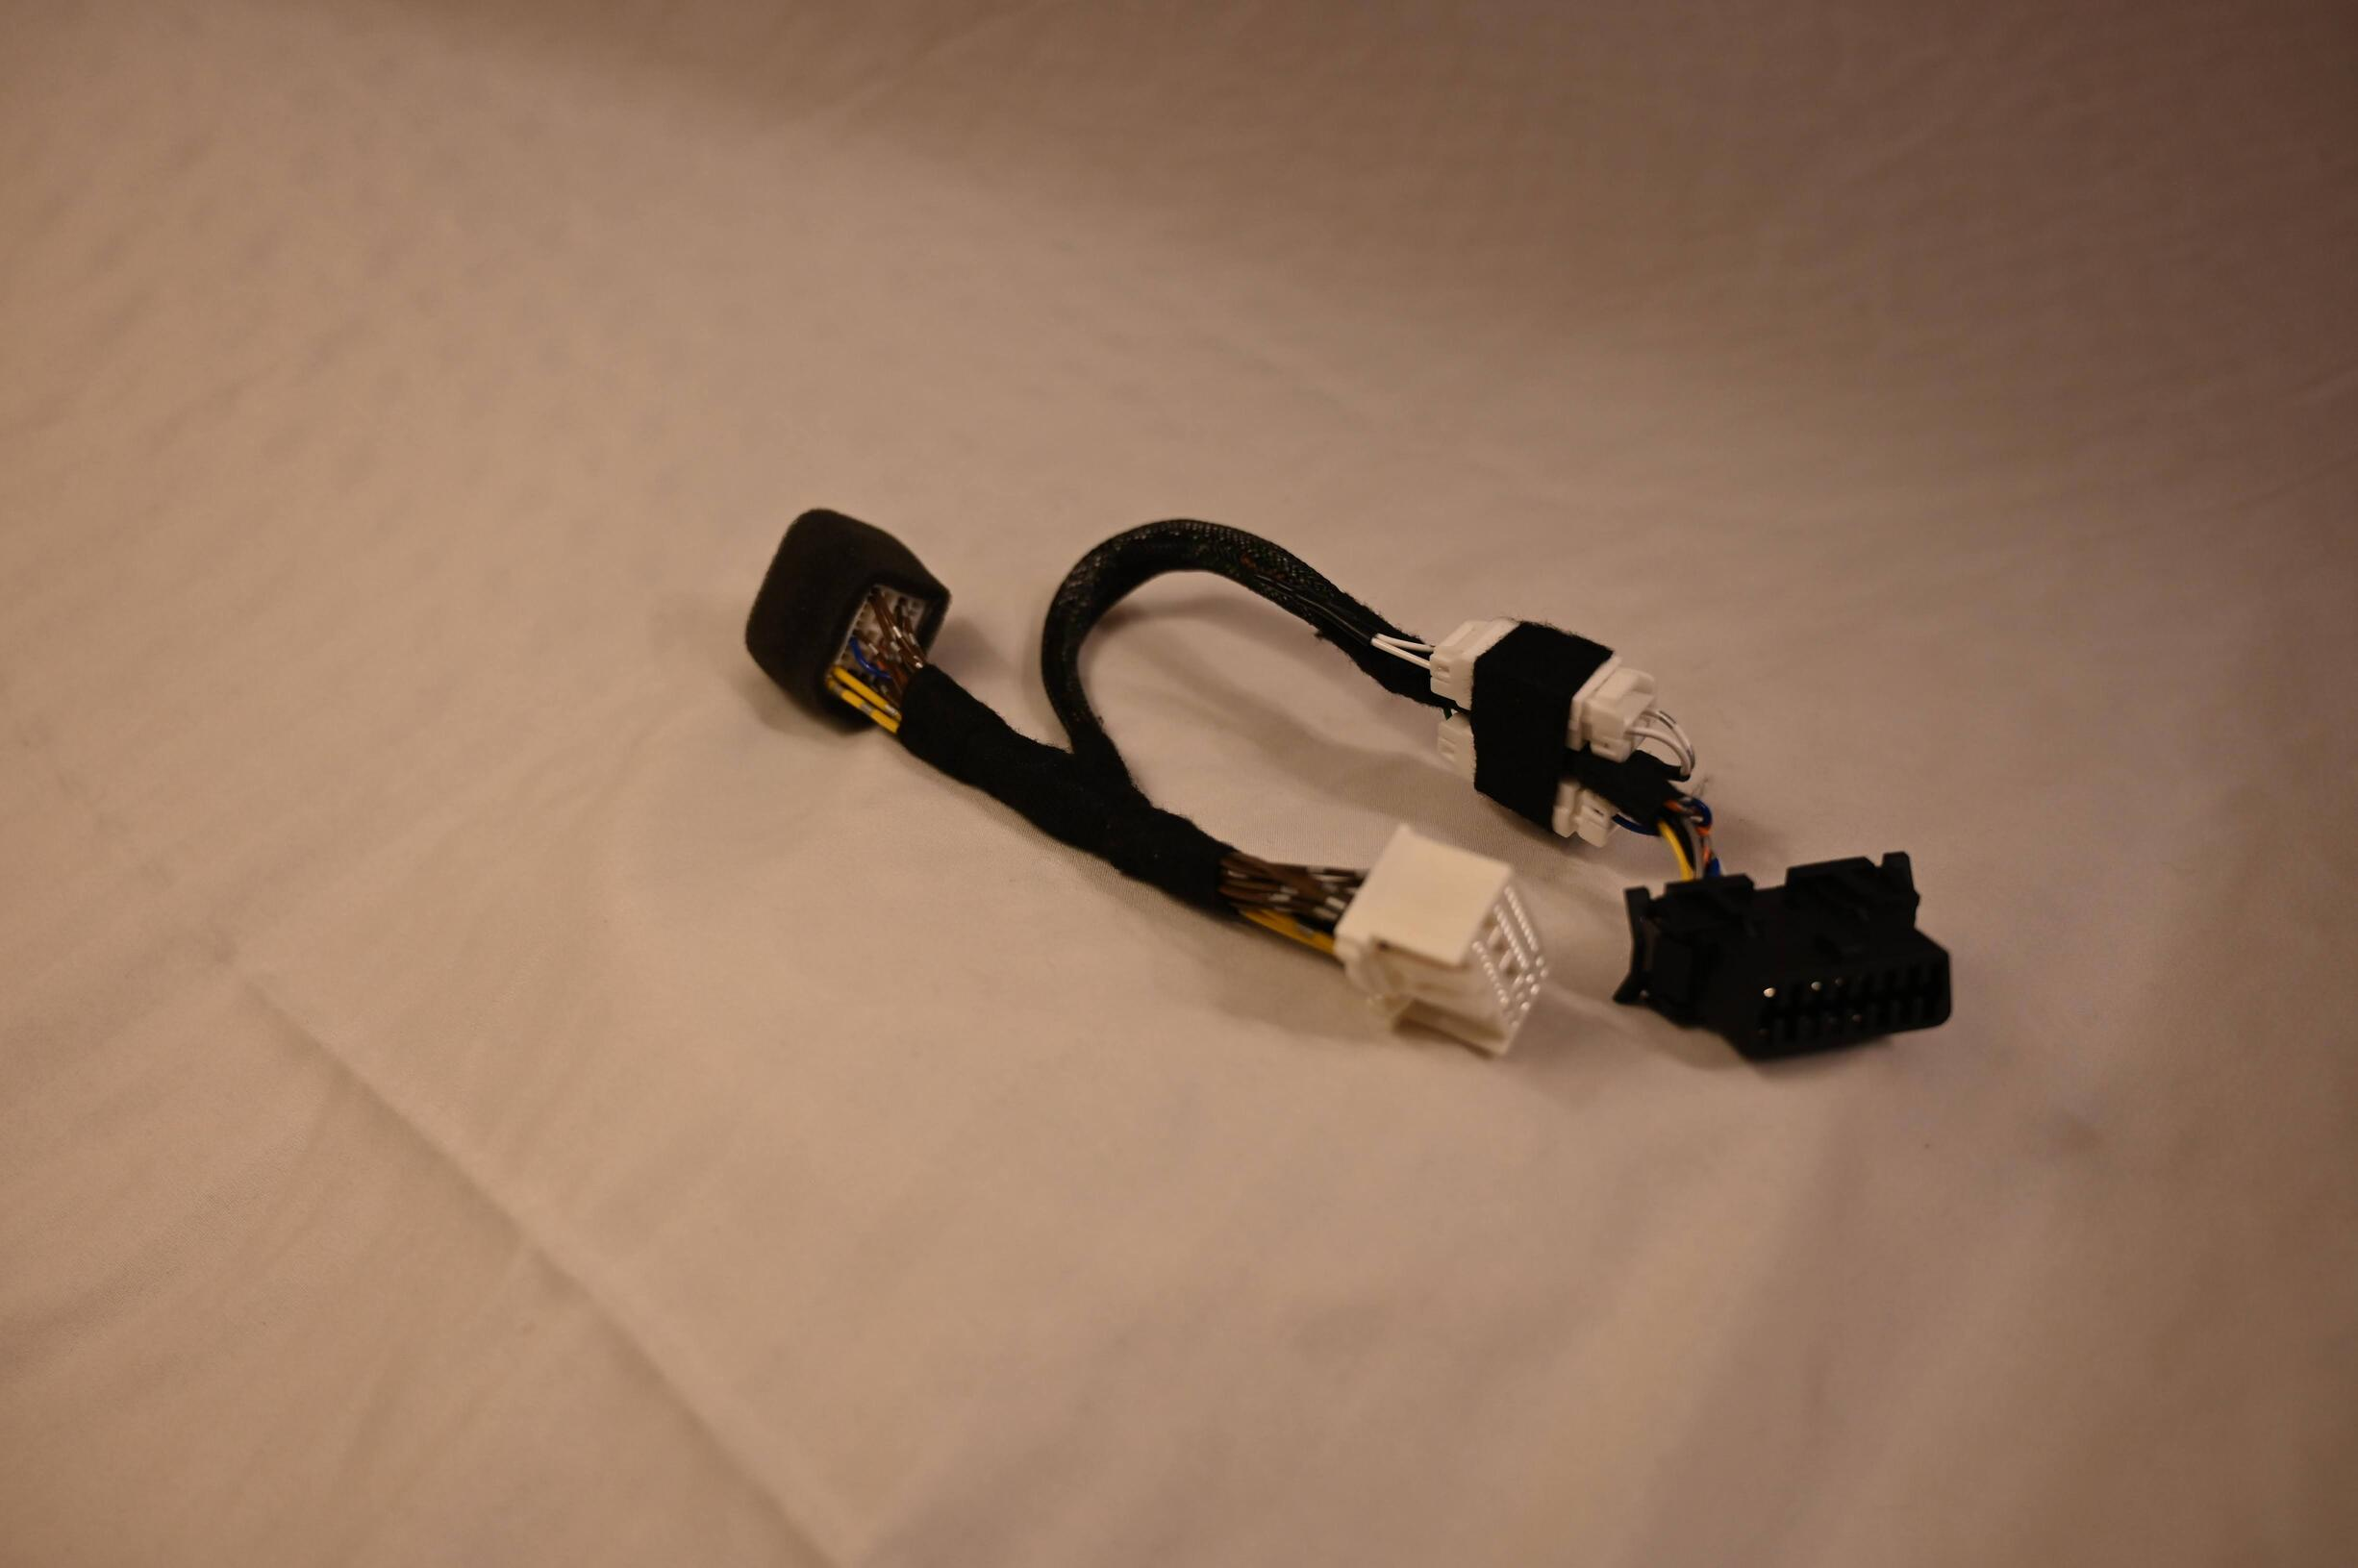
\includegraphics[height=1.95in]{../../../harnesses/head_unit_MITM/photos/whole_harness.jpg} } \\
%   \subfloat[]{\label{subfig:overview:trim}
%   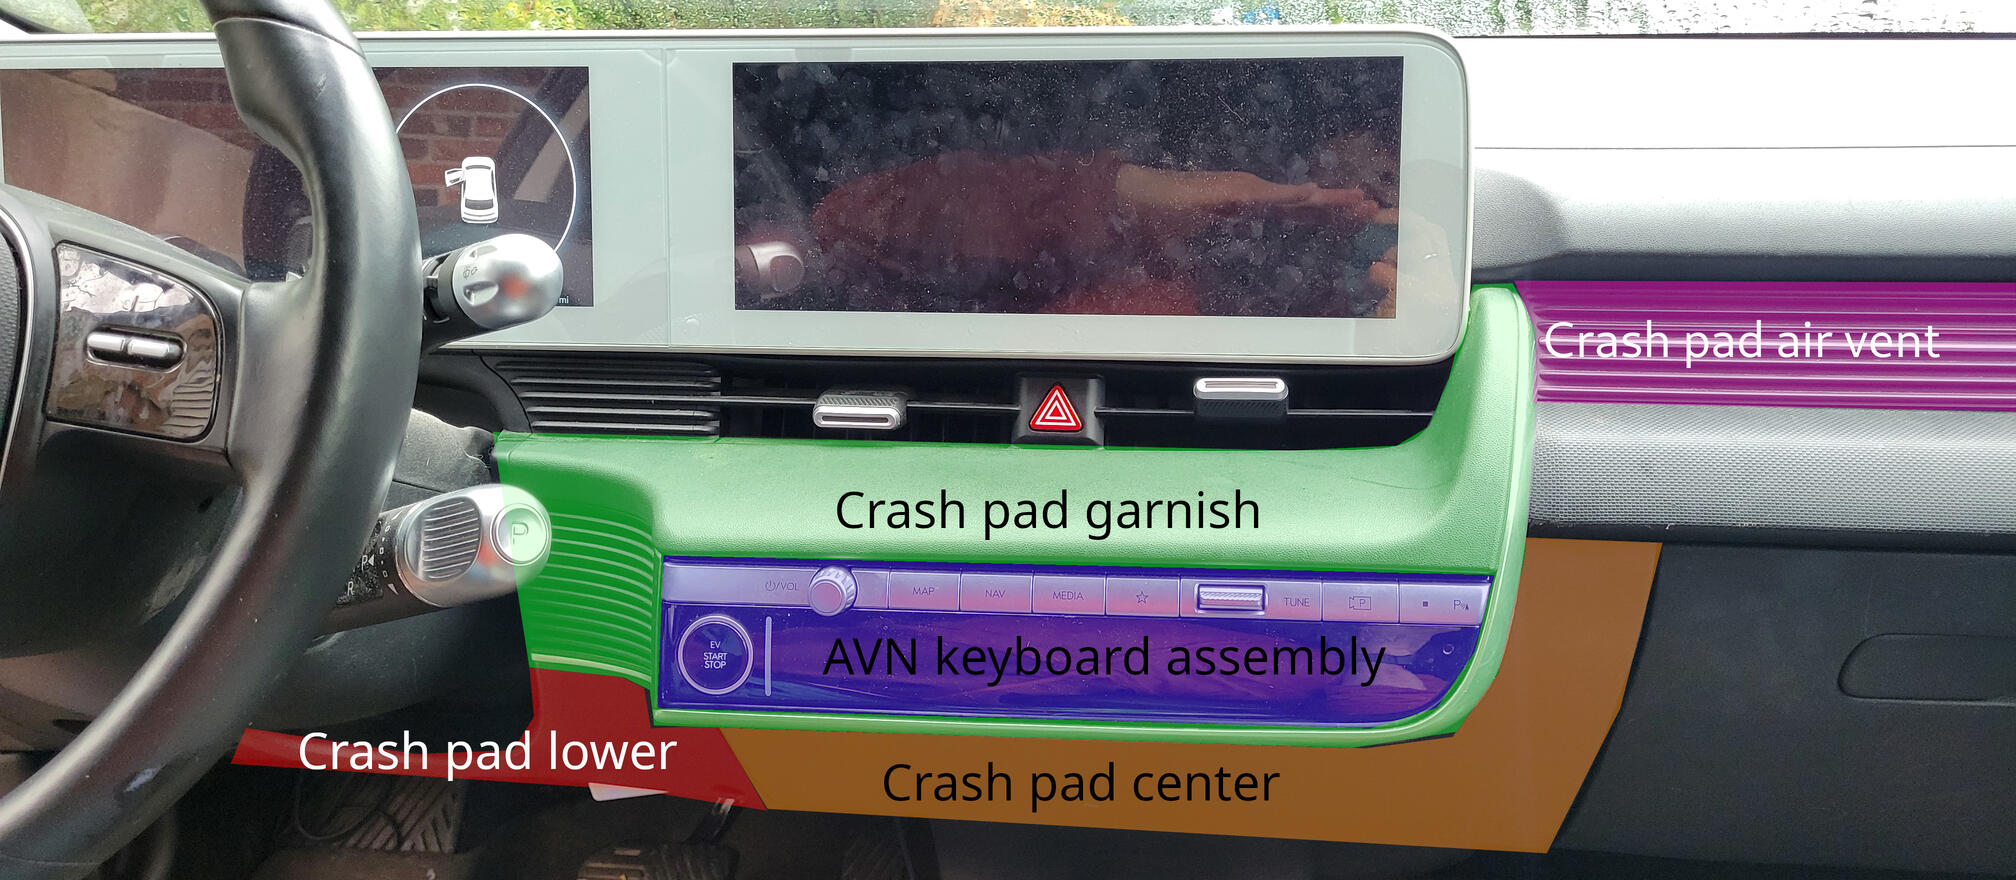
\includegraphics[width=6in]{photos/overview_labeled.jpg} }
%    \caption{(a) Man-in-the-middle harness. (b) Overview of trim panels involved. \label{fig:overview}}
% \end{figure}

\section{Introduction}
This guide describes the steps to install the selectable CAN harness into an Ioniq 5 ICU. See also \href{https://github.com/dragz/explorationsincarhacking/blob/main/articles/getting_past_the_secure_gateway/getting_past_the_secure_gateway.md}{these instructions} on identifying and acessing the ICU-H connector.

Necessary tools:
\begin{enumerate}
  \item 10mm socket or adjustable wrench for 12V battery
  \item Scissors
\end{enumerate}

Kit components:
\begin{enumerate}
  \item Selectable CAN harness
  \item WiCAN
  \item 60mm OBD mount bracket
  \item 70mm double-sided tape (two pieces included for redundancy)
  \item 4 zip ties
\end{enumerate}
  
\section{Step 1: Remove 12V Negative Terminal} \label{sect:0}
First, always disconnect the 12V battery before removing any electrical connectors! Removing a live electrical connector could cause a discharge and destroy a connector or ECU in your car.

Step-by-step instructions:
\begin{enumerate}
  \item Open hood (Figure \ref{subfig:12V:hood})
  \item Open frunk 
  \item Remove panel covering 12V (Figure \ref{subfig:12V:panel})
  \item Loosen nut on negative side with a 10mm socket (Figure \ref{subfig:12V:nut})
  \item Remove negative terminal (Figure \ref{subfig:12V:terminal})
\end{enumerate}

\begin{figure}[h]
  \subfloat[]{\label{subfig:12V:hood}
  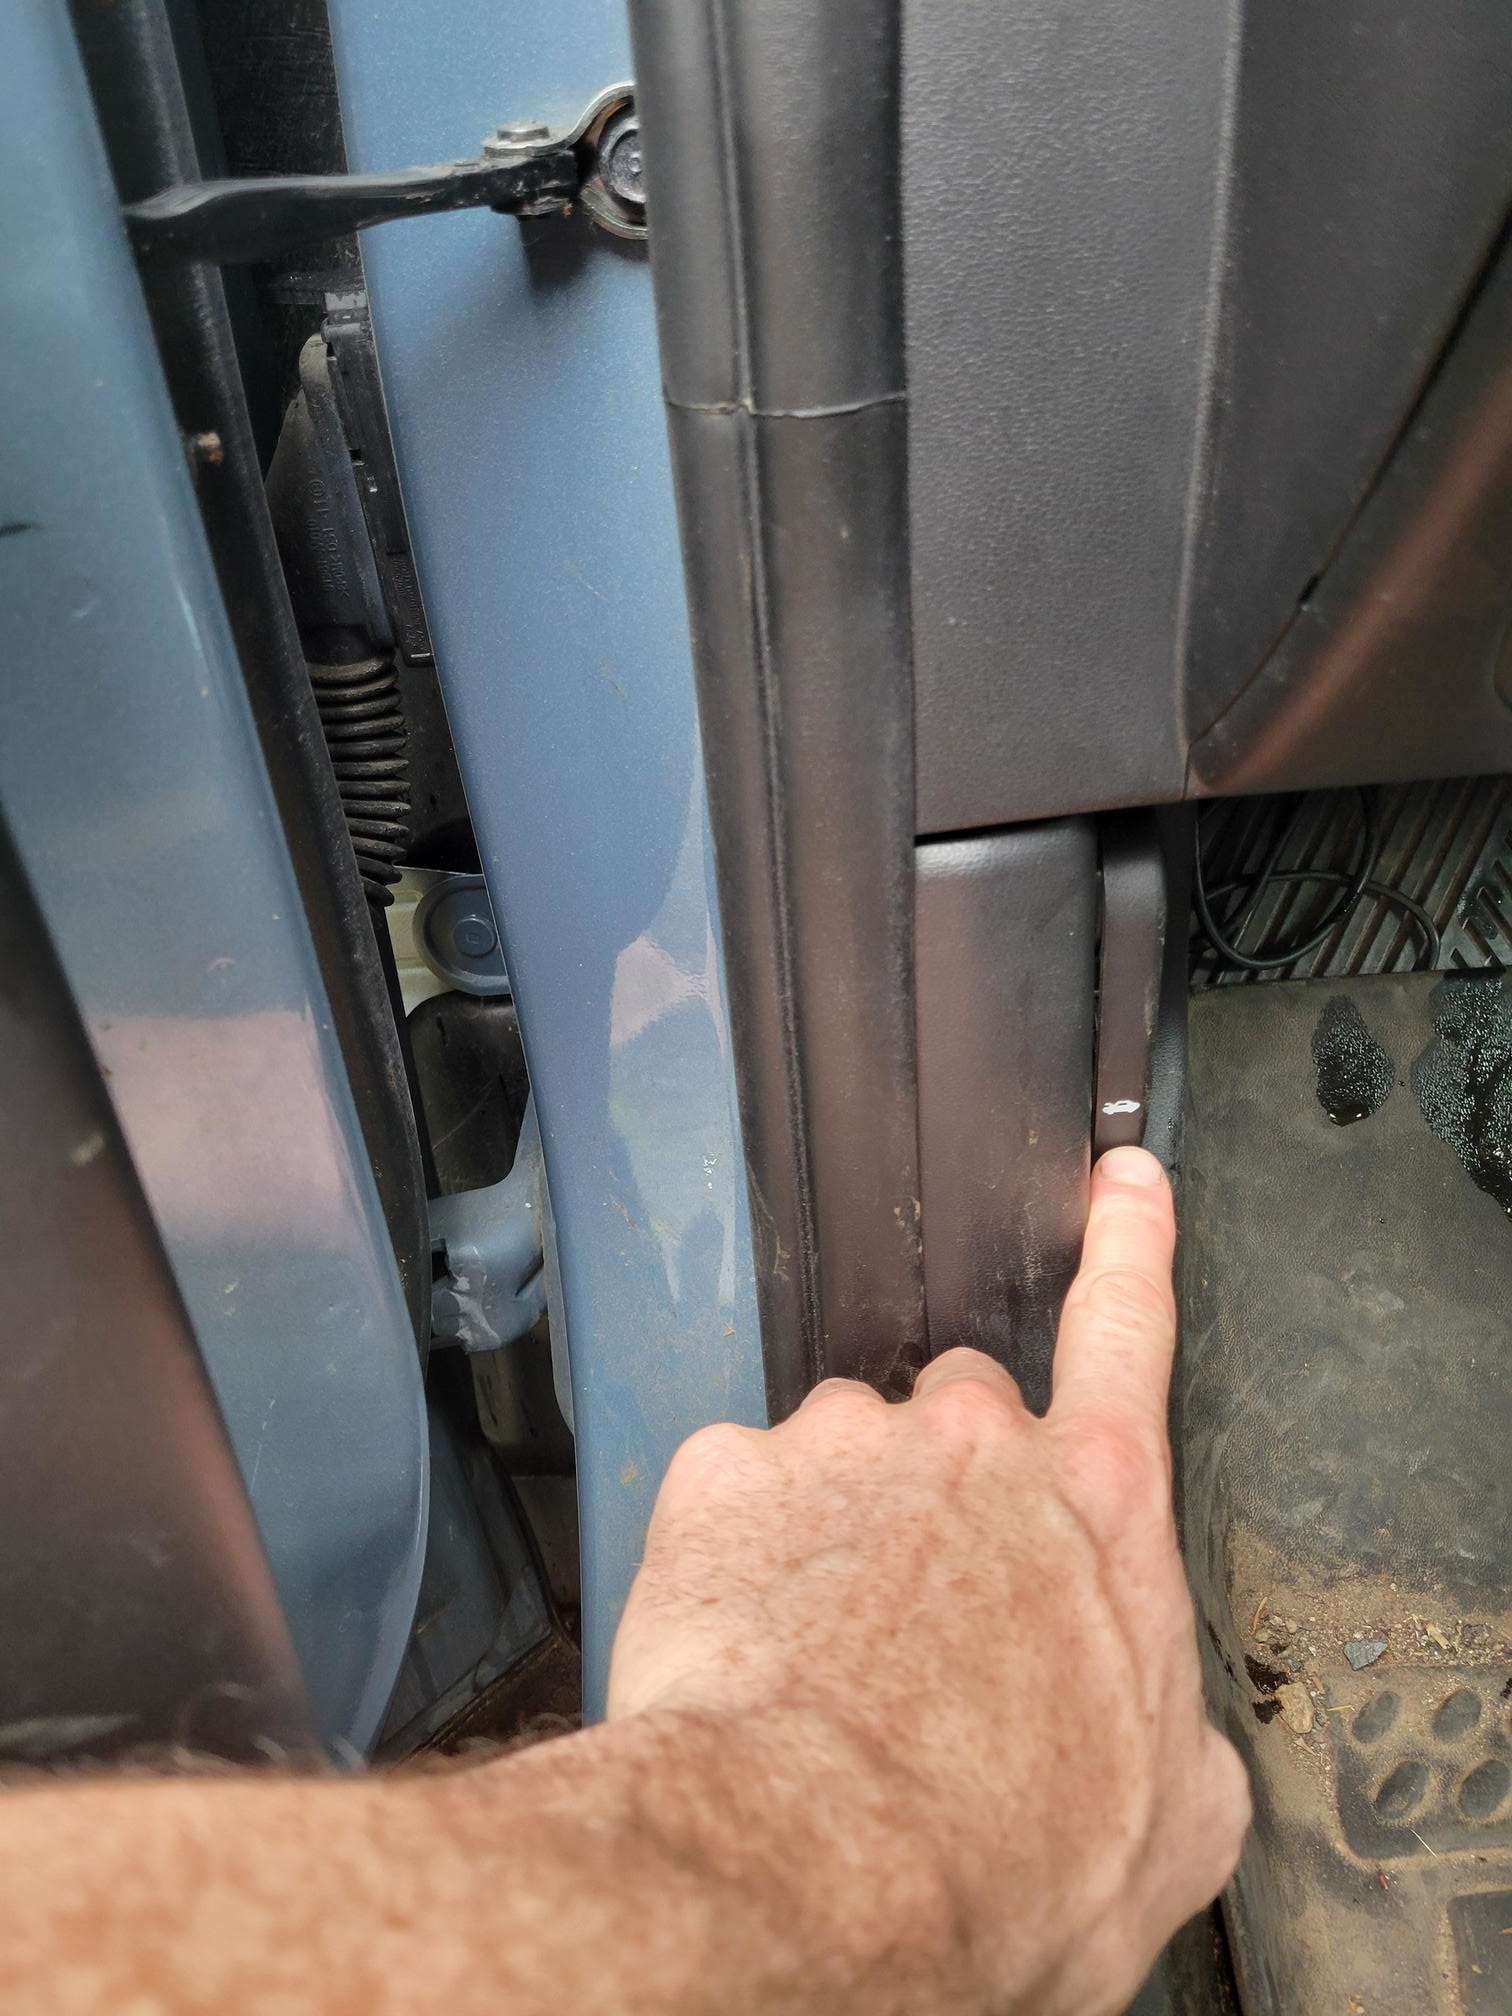
\includegraphics[height=1.5in]{photos/open_hood.jpg} } 
  \subfloat[]{\label{subfig:12V:panel}
  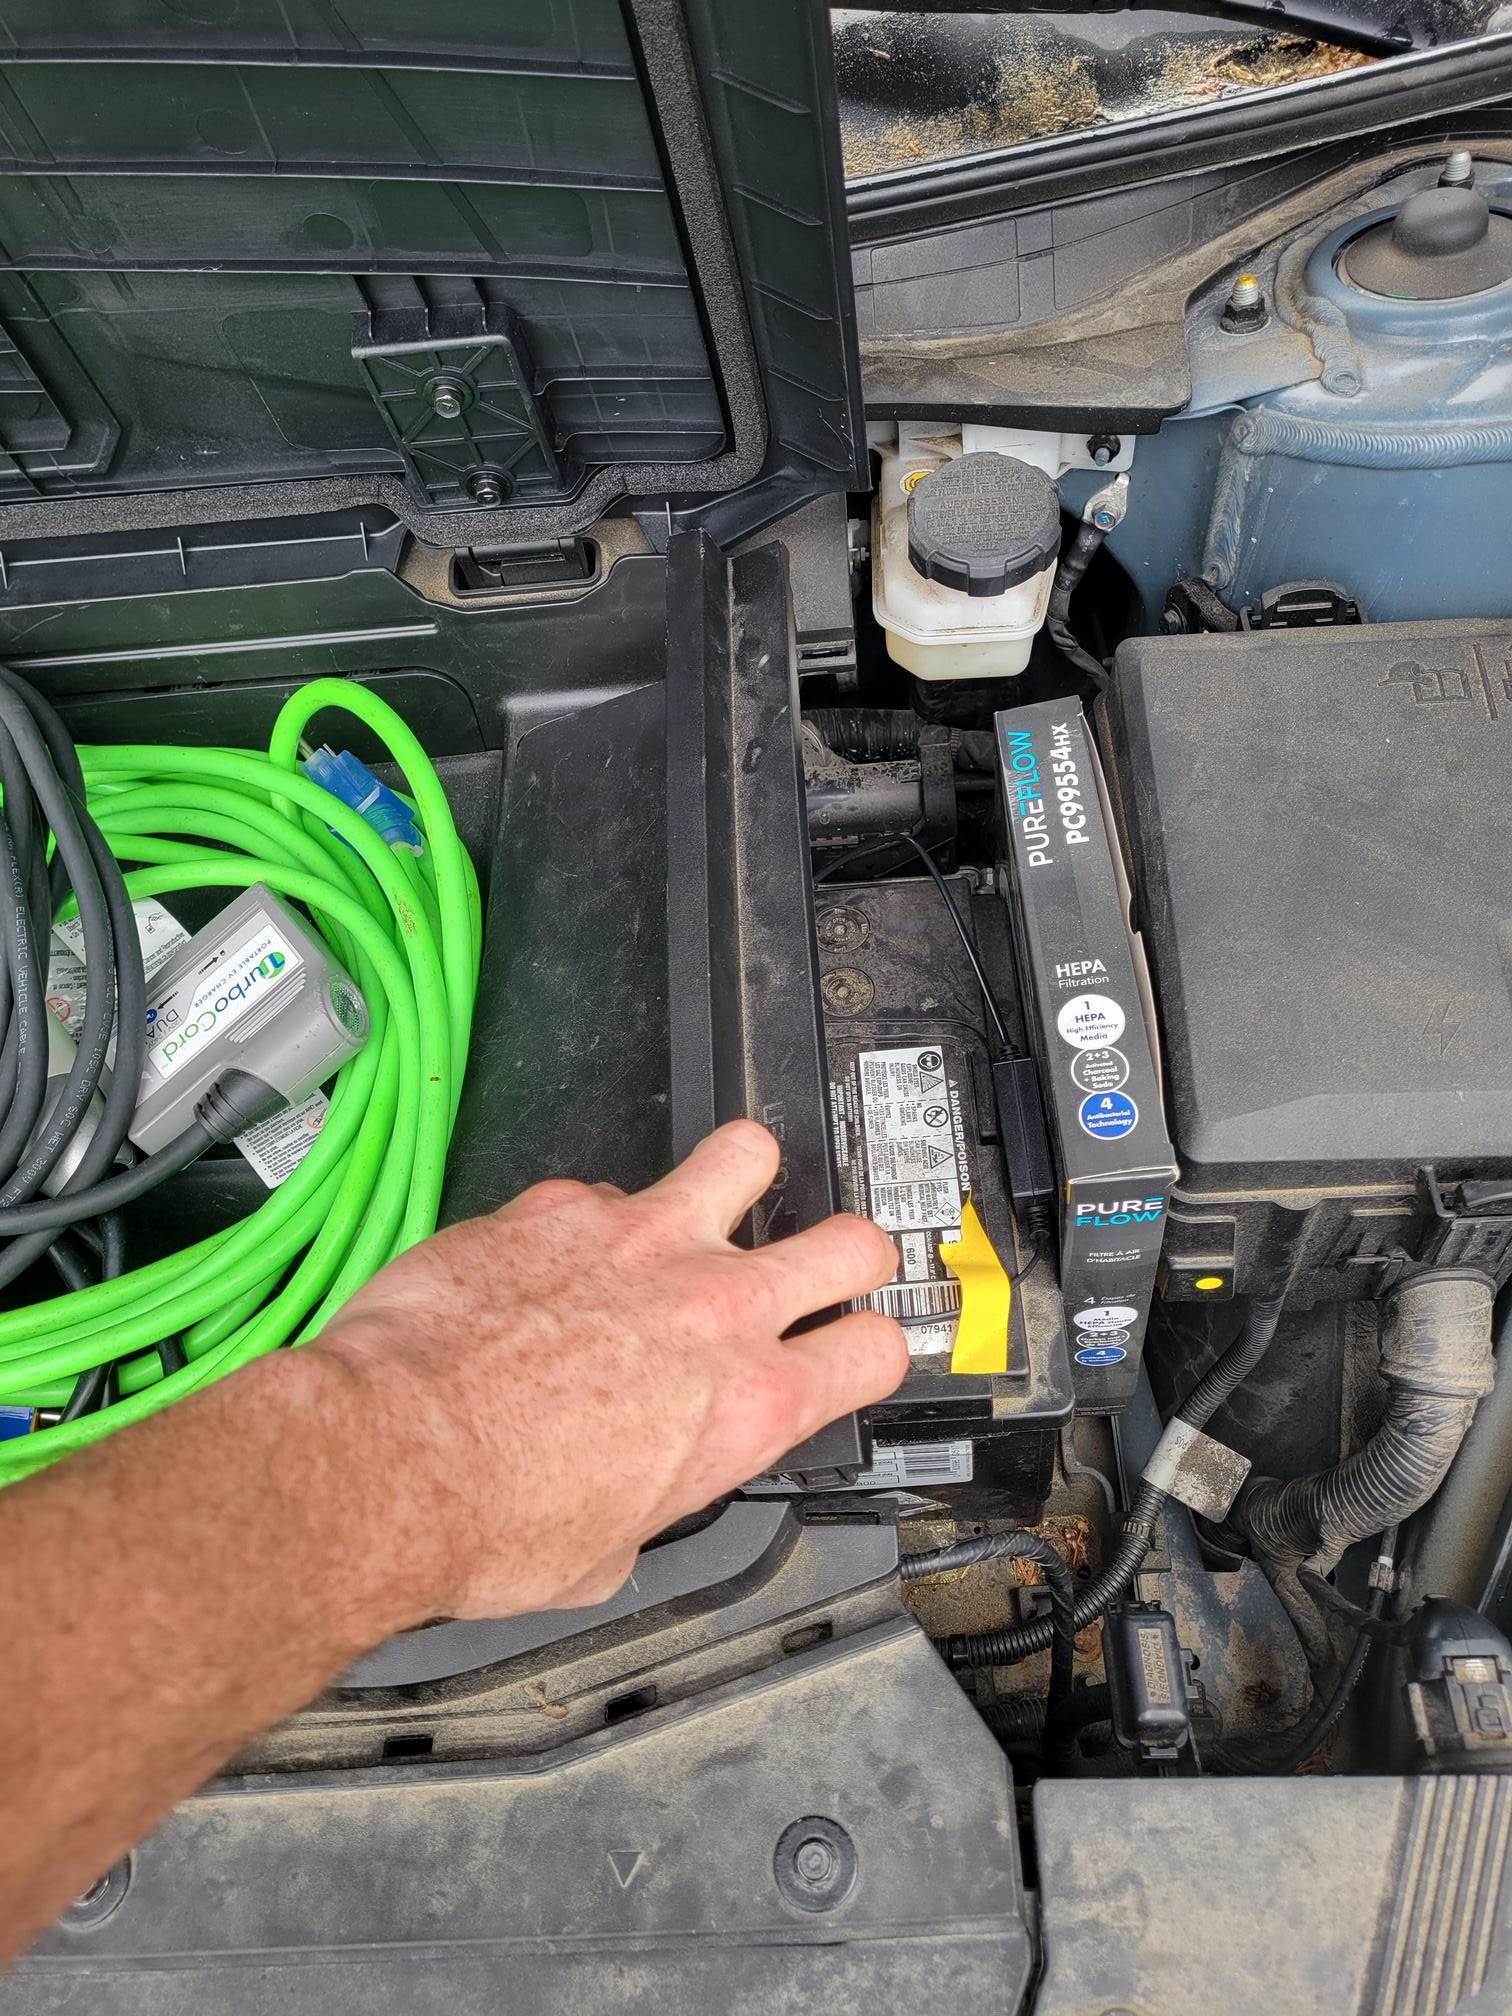
\includegraphics[height=1.5in]{photos/remove_panel.jpg} }  \\
  \subfloat[]{\label{subfig:12V:nut}
  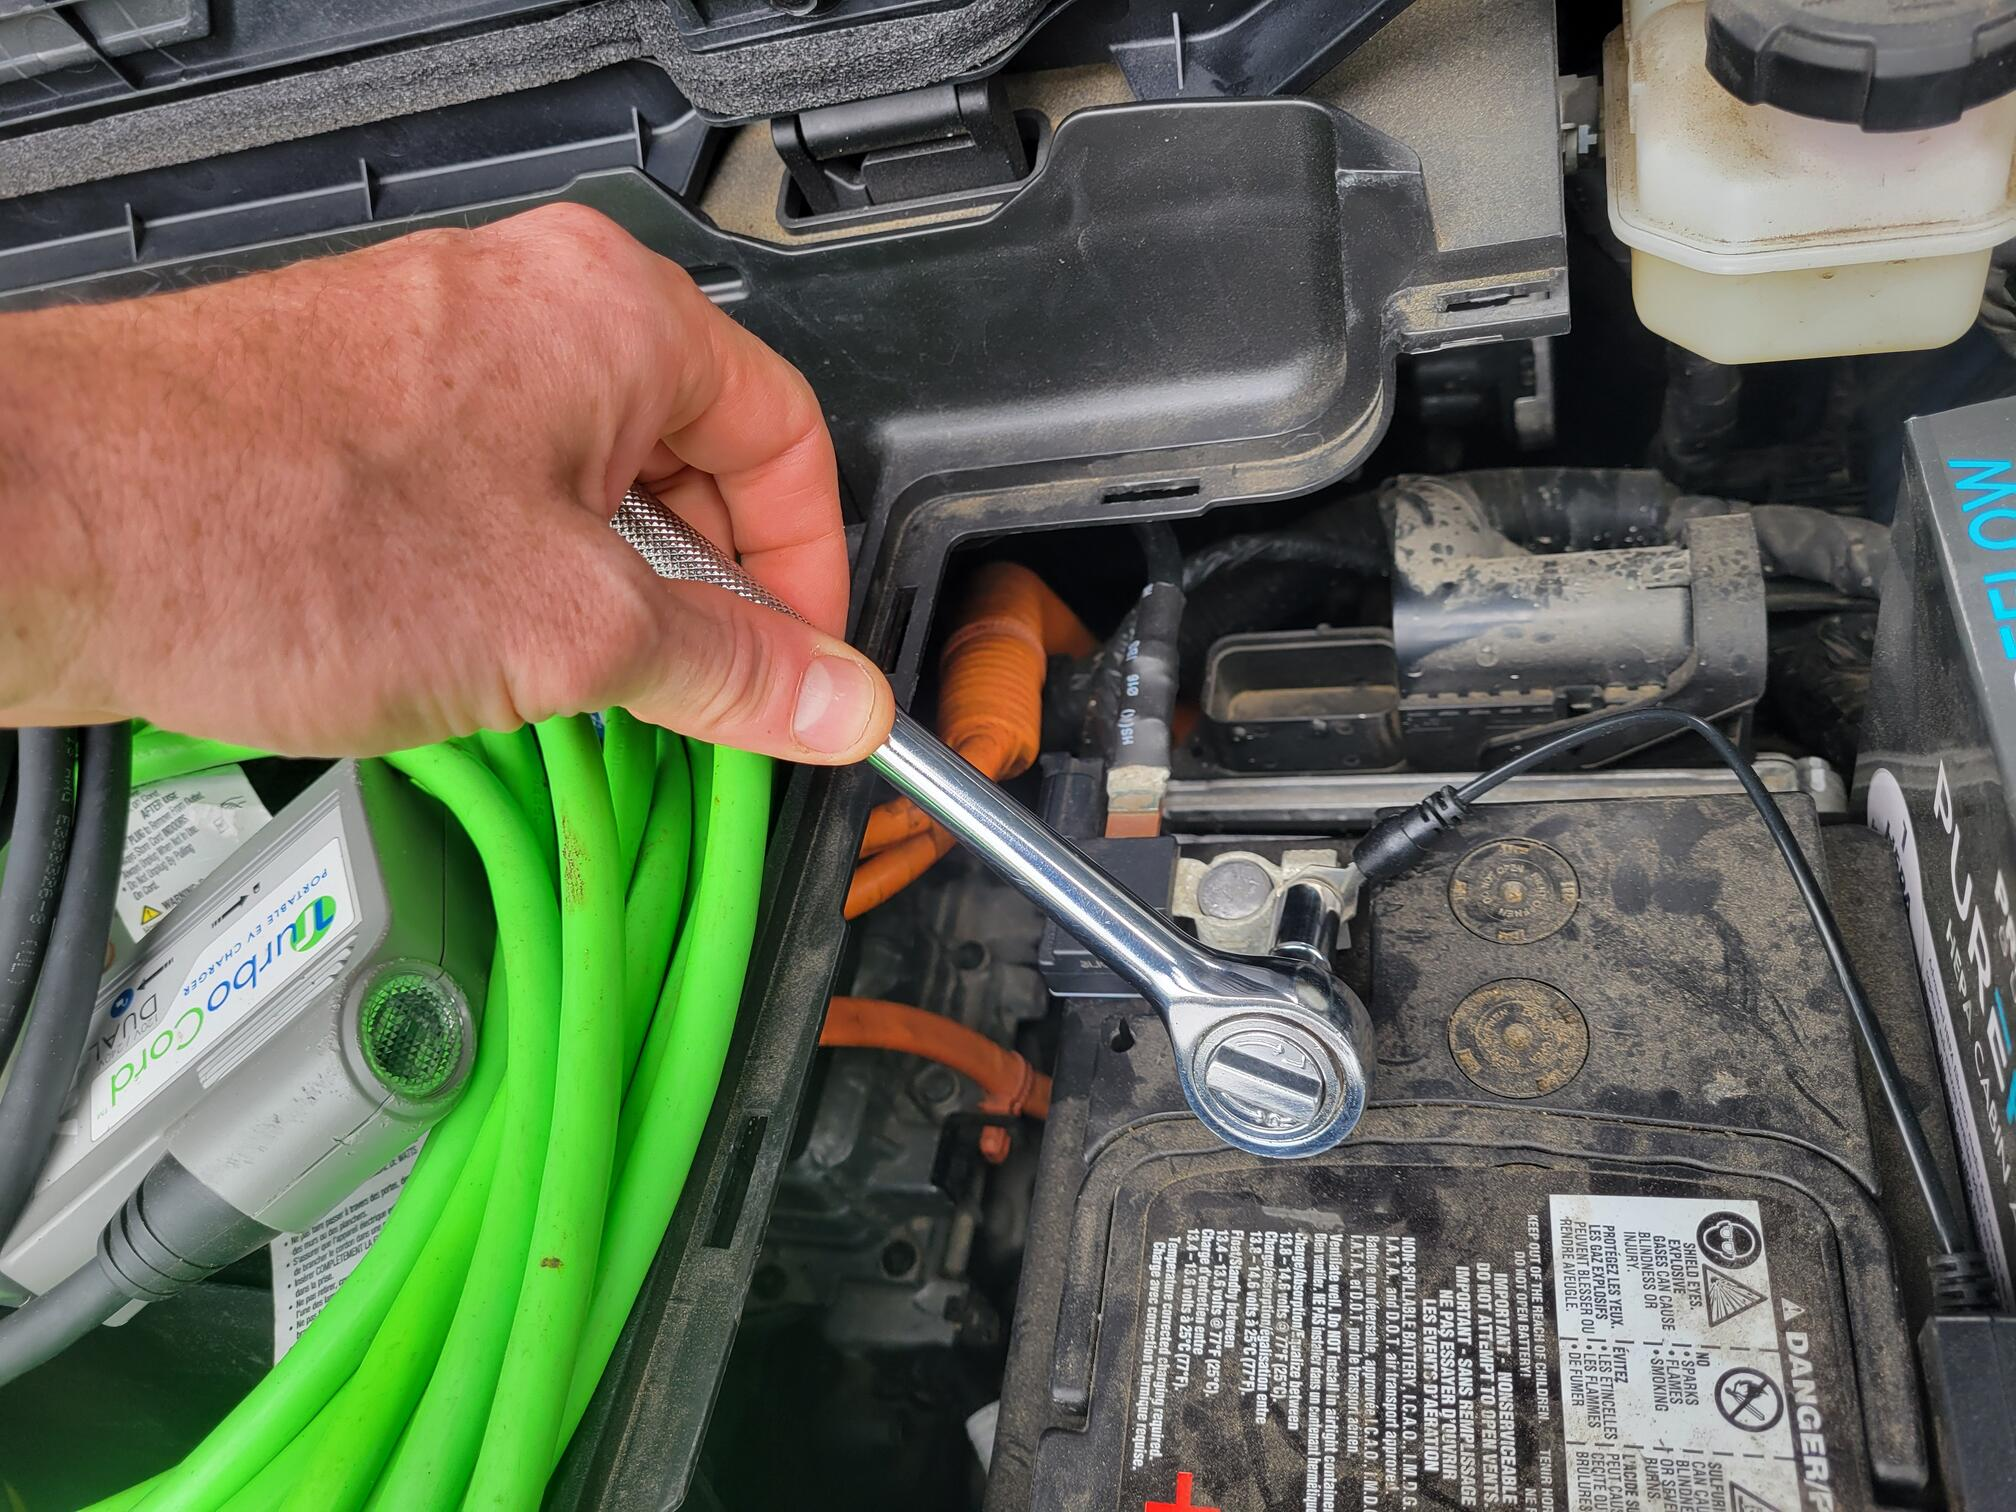
\includegraphics[height=1.5in]{photos/loosen_nut.jpg} } 
  \subfloat[]{\label{subfig:12V:terminal}
  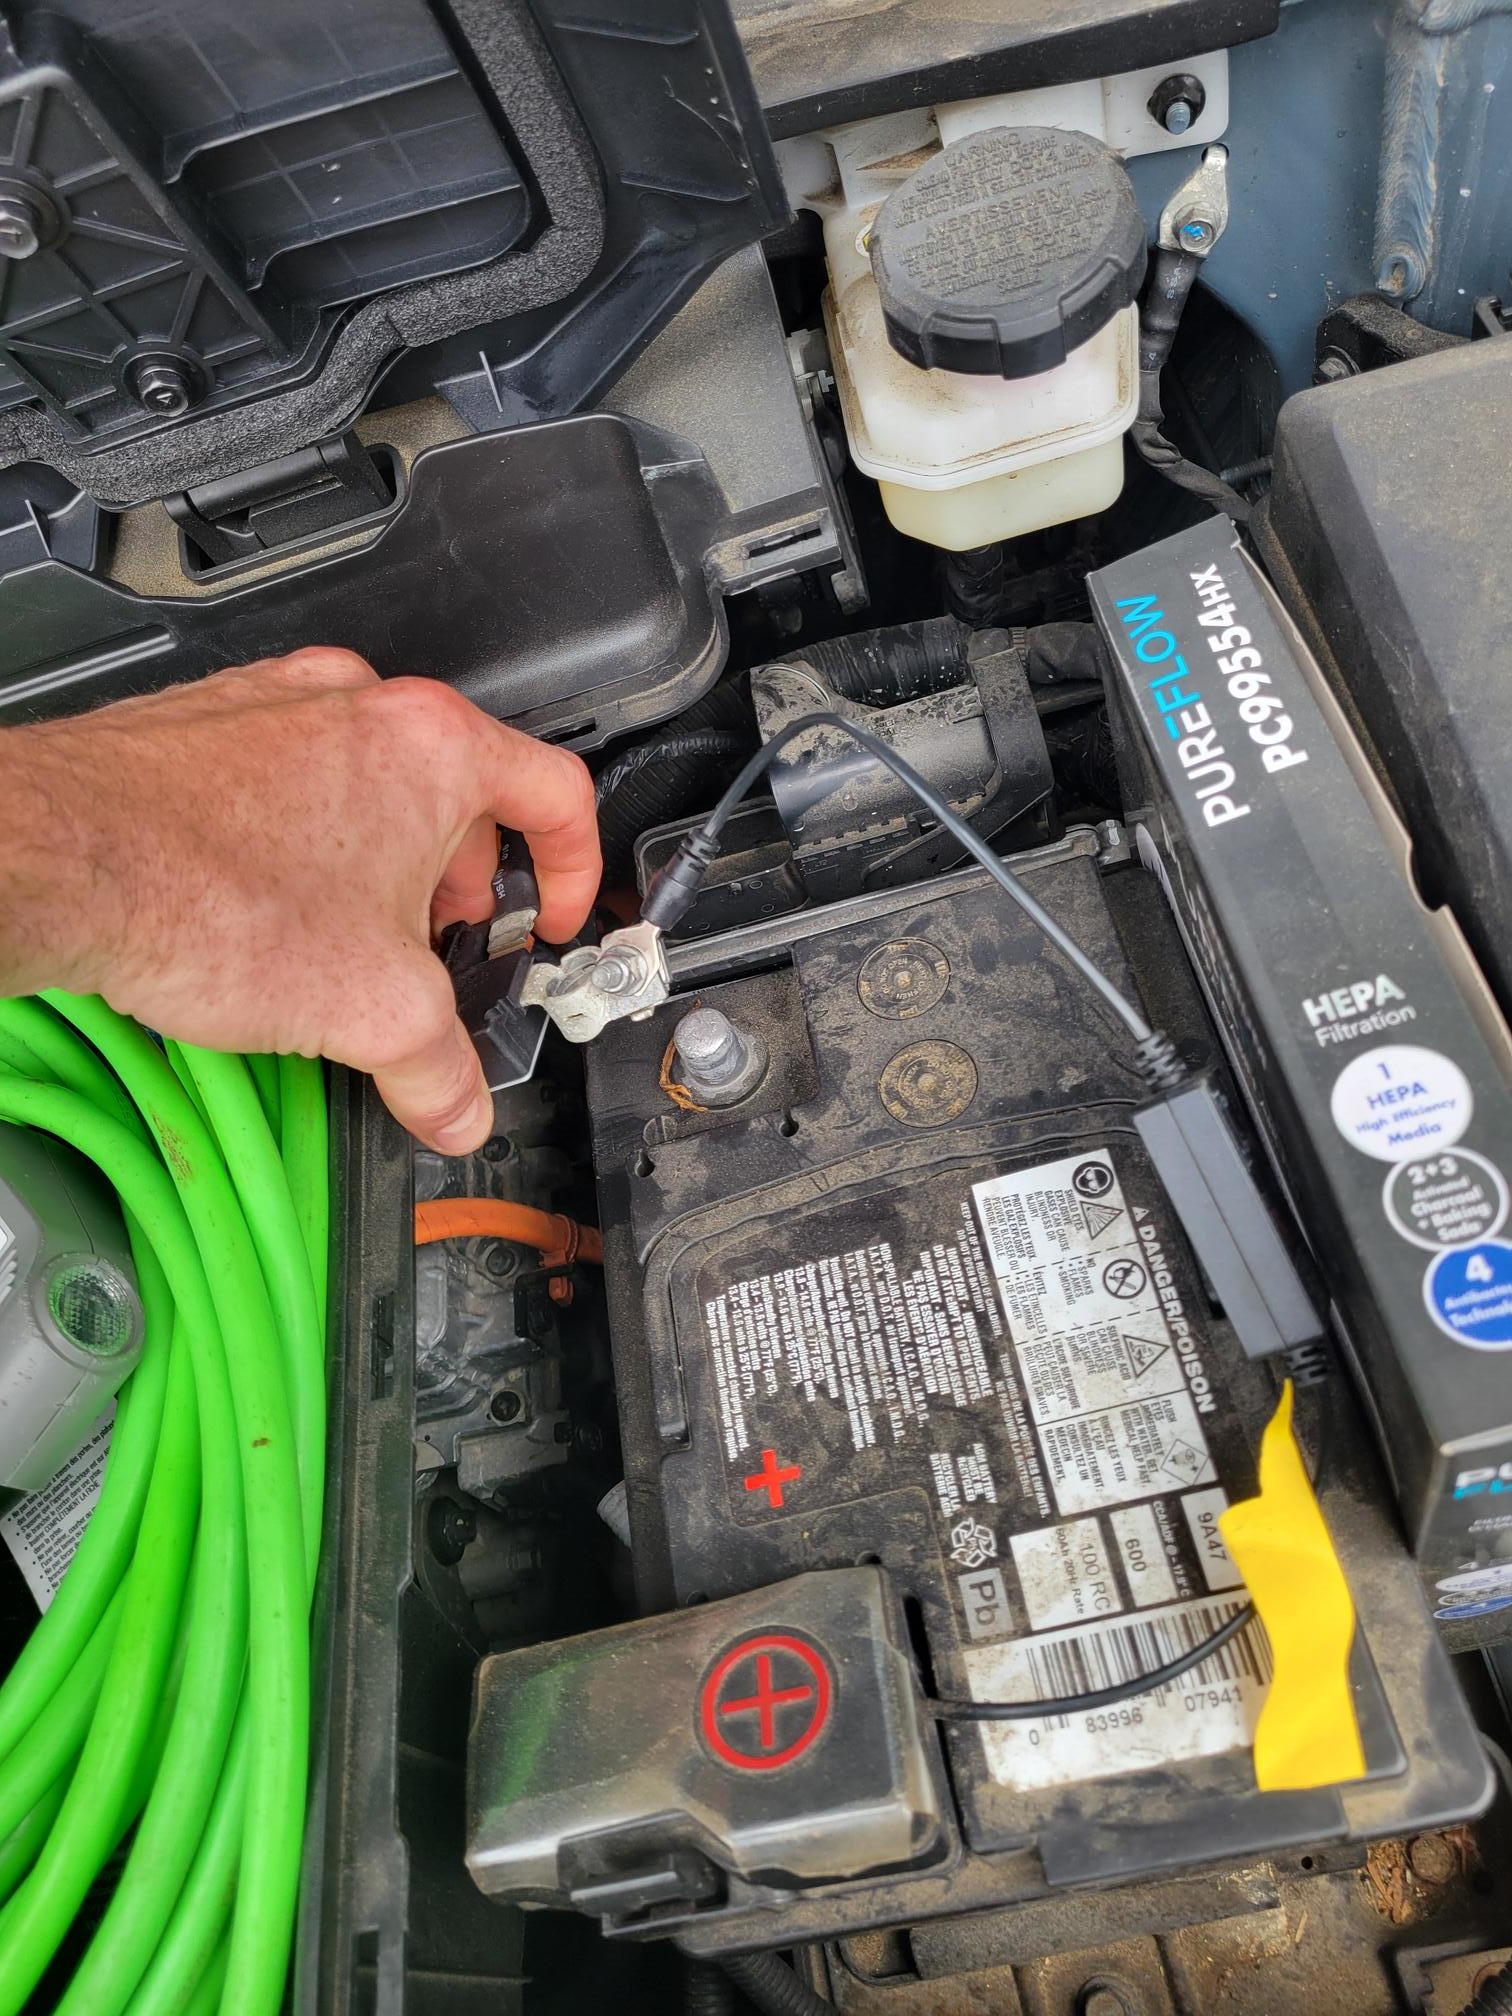
\includegraphics[height=1.5in]{photos/disconnect_terminal.jpg} } 
   \caption{(a) Open the hood. (b) Remove panel covering 12V. (c) Loosen nut on negative terminal. (d) Remove negative terminal. \label{fig:12V}}
\end{figure}

\section{Step 2: Harness Install} \label{sect:2}
This step will cover the installation of the harness into the ICU. 

Step-by-step instructions:
\begin{enumerate}
  \item (Optional) Remove ICU-H following \href{https://github.com/dragz/explorationsincarhacking/blob/main/articles/getting_past_the_secure_gateway/getting_past_the_secure_gateway.md}{these instructions}
  \item Install the fuse tap into spare 2 for always-on operation, or spare 1 for on-with-car-on operation (Figure \ref{subfig:harness:fusetap})
  \item Remove ICU-H connector (Figure \ref{subfig:harness:ICU-H})
  \item Insert the harness female side into the ICU 
  \item Insert the female connector you removed into the harness male side 
  \item Mount bracket on the side of the blue connector, so that the OBD face will point down (Figure \ref{subfig:harness:obd_mount})
  \item Insert the OBD port into the bracket
  \item Insert WiCAN into OBD port
\end{enumerate}

\begin{figure}[h]
  \subfloat[]{\label{subfig:harness:fusetap}
  \includegraphics[height=1.5in,angle=0]{photos/fuse_tap_in_wrong.jpg} } 
  \subfloat[]{\label{subfig:harness:ICU-H}
  \includegraphics[height=1.5in,angle=0]{photos/icu-h_harness_in.jpg} }  
  \subfloat[]{\label{subfig:harness:obd_mount}
  \includegraphics[height=1.5in,angle=0]{photos/obd_mounted_icuh.jpg} } 
   \caption{(a) Fuse tap doubled with dashcam fuse tap on spare 2. Note that this will not work as depicted and requires a second fuse on the lower fuse tap. (b) ICU-H (green arrow) with harness installed; male harnesss connector (red arrow) mated with original female connector. (c) OBD port mounted on bracket. \label{fig:harness}}
\end{figure}

\section{Step 3: Clean up} \label{sect:4}
Reconnect 12V battery negative terminal. The WiCAN should immediately show a blue light. \href{https://meatpihq.github.io/wican-fw/config/wifi}{Change your WiCAN password!}. You can connect you your WiCAN directly by finding a WiFi network named 'WiCAN\_xxxxxxx' and going to \href{http://192.168.80.1/}{http://192.168.80.1/} in your browser.
\appendix 
\bibliographystyle{apsrev4-1}
\bibliography{stemh_model}{}
\end{document}